\chapter{From edges to contours} % - Current State-of-the-Art}
\label{Chapter3}
\settocdepth{subsubsection}

In this chapter we review a recent segmentation method, introduced in~\cite{Arbelaez09} and further developed %refined 
in ~\cite{Arbelaez11}.

\section{gPb-OWT-UCM algorithm pipeline}
\begin{figure}[ht!]
\centering
 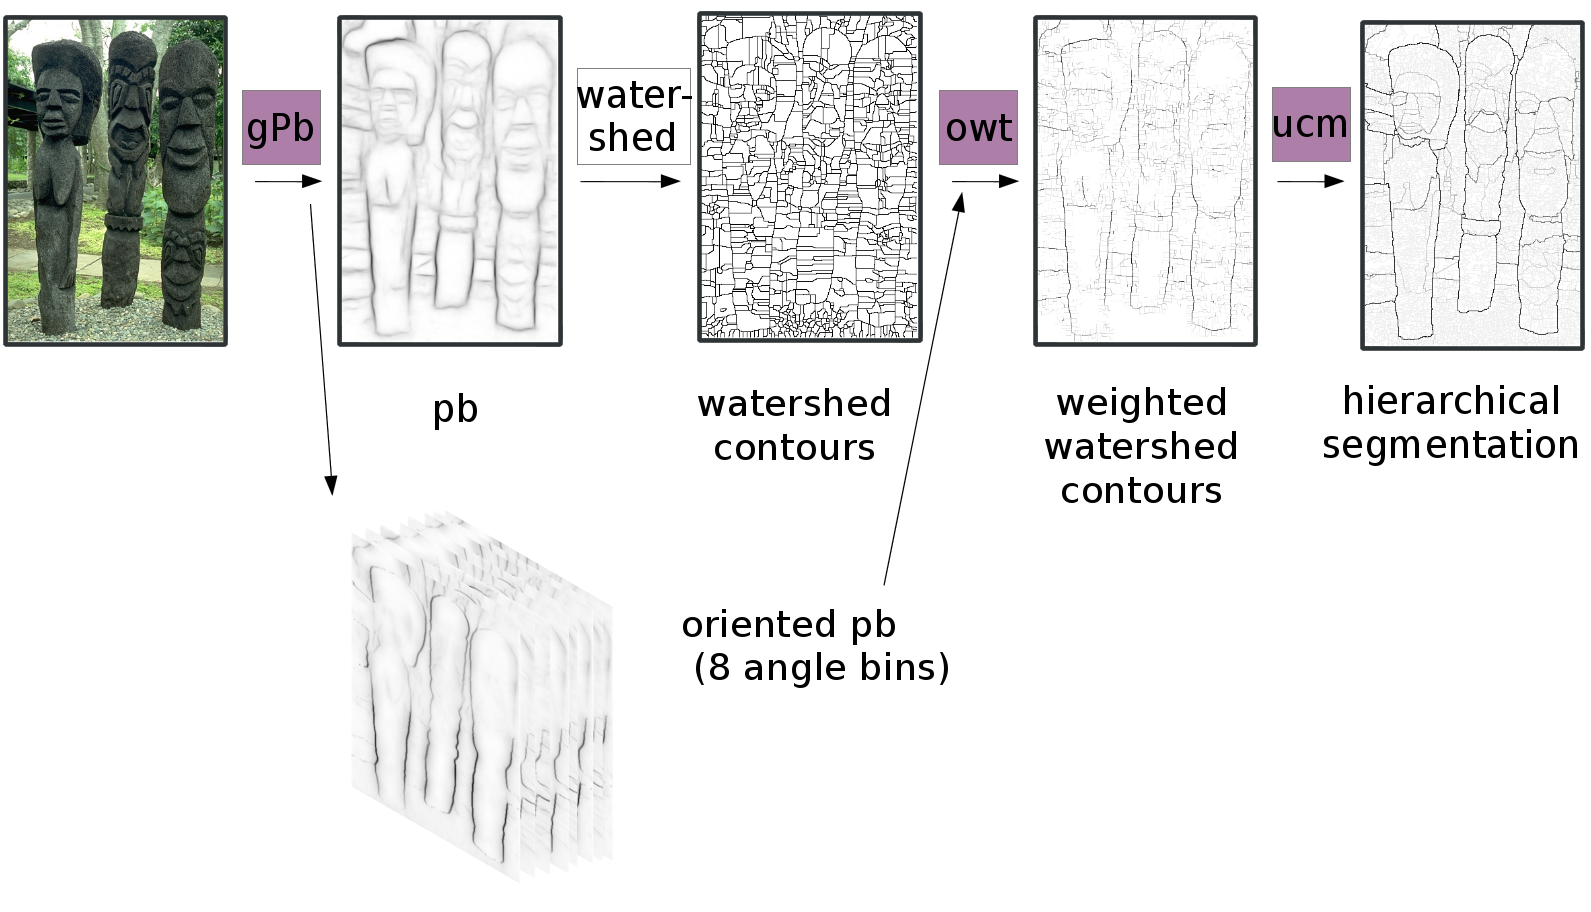
\includegraphics[width=1\textwidth]{images/gPb-OWT-UCM/gPb-OWT-UCM_pipeline.png}
\caption{gPb-OWT-UCM algorithm. We have expanded the pipeline to explicitly include the ``watershed transform'' operation and its output - watershed contours.}
\label{fig:gPb-OWT-UCM-pipeline}
\end{figure}

\subsection{First stage of the pipeline - edge detection} % gPb
The gPb algorithm utilises local cues - colour, brightness and texture to build features. Those are then globalised using spectral clustering. Multiple-scale approach gives competitive edge detection results.
% TODO discuss multiple orientations; put image

\textbf{Quantised oriented probability of boundary}
\subsection{Second stage of the pipeline - weighting the watershed} % OWT
\subsubsection{Watershed}
\label{sec:ch3-watershed}
The watershed transform is a basic morphological operation~\cite{beucher1992morphological} used to produce an image segmentation. Given an intensity %a greyscale 
image as an input, it would output watershed \textit{segments} (\textit{regions}), which are complimentary to the watershed \textit{pixels} (\textit{contours}). The latter are by construction closed contours. A well-known shortcoming of the watershed transform is that the 
segmentation produced by it is an oversegmentation, due to a catchment basin forming around every regional minimum.

Unlike ``Seeded region growing''~\cite{adams1994seeded}, the watershed algorithm does not require as input any initial seeds for forming watershed regions.

Note that the watershed algorithm only provides a single segmentation, but does not build a hierarchy. %but not weights to them, hence, 
Najman~\etal~\cite{najman1996geodesic} offer a way to obtain a hierarchy of segmentations from the watershed pixels, which unfortunatelly involves the selection of a set of markers.

The watershed transform is a suitable intermediate step in obtaining hierarchical segmentation from edge detection output, since it provides a straightforward means to close contours. The probability of boundary is a one-channel image and can therefore be used as an input to the watershed transform. Thus, the locations of the watershed contours constitute a binary image indicating the higest level of recall in the context of the Precision-Recall framework of~\cite{Arbelaez11}. % (c.f. edge map)

In practice the vanilla watershed implementation in MATLAB~\cite{MATLABwatershed} is used, with 8-connected neighbourhood for the regions.

\settocdepth{section}
\subsubsection{Oriented watershed transform (OWT)}
\settocdepth{subsubsection}
\label{sec:ch3-OWT}
% TODO define watershed arcs

\subsection{Third stage of the pipeline - UCM}
\label{sec:ch3-UCM}
% TODO
The {\it Ultrametric contour map} (UCM) was introduced in \cite{Arbelaez2006boundary}. It constitutes a convenient datastructure for the representation of a hierarchical segmentation. 

The map is constructed by agglomerative clustering of regions based on the weight of their common boundary. It represents a tree, at the leaves of which are the superpixels at the highest level of detail. Going up the tree merges regions. It is an real-valued image (see \fref{fig:sub:segmentation-ucm} and \fref{fig:sub:segmentation-ucm-cc}) in which every region boundary is weighted by its scale of disappearance.

% Multiple segmentatons, but going up the UCM coarsens the segmentation.

% TODO give the algorithm in an appendix
% coarse-to-fine
% agglomerative clustering

\section{Limitations of the gPb-OWT-UCM} %quantisation} % or drawbacks, don't say 'flaws'
Quantisation